\par The longitudinal momentum of the proton constituents during $pp$ collisions at the LHC 
is not known. Rather, the total transverse momentum of these constituents is expected to be 
insignificantly smaller than the longitudinal momentum. So, the total transverse momentum 
before a $pp$ collision can be taken as zero. Due to conservation of momentum, it should also 
be zero after the collision. In other words, transverse momentum imbalance, also known 
as {\it missing transverse energy (MET, or $\boldsymbol{\met}$)}, is expected to be zero if all decay products were 
detectable by the ATLAS detector.  

\par Neutrinos leave no signature in the ATLAS detector; they are invisible. 
Their presence is inferred by the presence of $\boldsymbol{\met}$, whose $x$ and $y$ components 
are defined as 

\begin{dmath}
E^{\text{miss}}_{x(y)} = E^{\text{miss},e}_{x(y)} + E^{\text{miss},\gamma}_{x(y)} +E^{\text{miss},\tau}_{x(y)} +E^{\text{miss,jets}}_{x(y)} + E^{\text{miss},\mu}_{x(y)} + E^{\text{miss,soft}}_{x(y)}, 
\label{eq:metDef}
\end{dmath} 

where each term is either the negative sum of \pt components, or the negative sum of cell energies, weighted according to their position in $\eta$ and $\phi$ as follows : 

\begin{equation}
\begin{aligned}
E^{\text{miss,term}}_{x} = \sum_{i=1}^{N^{\text{term}}_{\text{cell}}}E_i\sin\theta_i\cos\phi_i  & \text{ and} & 
E^{\text{miss,term}}_{y} = \sum_{i=1}^{N^{\text{term}}_{\text{cell}}}E_i\sin\theta_i\sin\phi_i.  
\end{aligned}
\end{equation}

The $E^{\text{miss,soft}}_{x(y)}$ term is called the {\it soft term}, and the sum of the other terms is collectively called 
the {\it hard term}. Reconstruction of the soft and hard terms differs slightly between 
Run I and Run II, as discussed in Sections~\ref{sec:runImet} and~\ref{sec:runIImet}.
To avoid ambiguities in the detector signals used to construct the physics objects used in the hard term, 
a priority list is defined. Electrons, having the highest purity, are considered first, followed by 
photons, hadronic $\tau$ leptons, muons and finally jets. This means that objects low in the 
priority list are removed from the list if they share detector signals with objects higher in the 
priority list.  

\par Approximating the neutrino masses with zero, $\boldsymbol{\met}=\boldsymbol{p_{\mathrm T}^{\mathrm{miss}}}$. These 
two quantities are therefore used interchangeably in this text.  

\par The magnitude of $\boldsymbol{\met}$ is then   

\begin{equation}
\met = \sqrt{(E^{\text{miss}}_x)^2 + (E^{\text{miss}}_y)^2}
\end{equation}
 
and its $\phi$ direction is 

\begin{equation}
\phi^{\text{miss}} = \arctan(E^{\text{miss}}_y,E^{\text{miss}}_x).
\end{equation}   

The scalar sum of the \pt\ of all the objects in the event is then 

\begin{equation}
\sum\eT = \sum_{i\in\text{hard}}p_{\text{T,i}} + \sum_{j\in\text{soft}}p_{T,j}.
\end{equation}

\subsection{Run I Reconstruction}
\label{sec:runImet}
\par While the hard term in Run I reconstruction is formulated as in Equation~\ref{eq:metDef}, the soft term is formulated as 
 
\begin{dmath}
E^{\text{miss,soft}}_{x(y)} = E^{\text{miss,softjets}}_{x(y)} +E^{\text{miss,CellOut}}_{x(y)} + (E^{\text{miss,calo},\mu}_{x(y)}),
\label{eq:softmetDef}
\end{dmath} 

where the parentheses on one of the terms hint towards a caveat. 

\par $E^{\text{miss},e}_{x(y)}, E^{\text{miss},\gamma}_{x(y)}$ and $E^{\text{miss},\tau}_{x(y)}$ are calculated from cells in clusters 
associated with electrons, photons and hadronic $\tau$ leptons respectively. The electrons and photons are calibrated at the 
electromagnetic scale, while the hadronic $\tau$ leptons are calibrated with the LCW scheme. 
Electrons, photons and hadronic $\tau$ leptons used for this calculation are required to have at least 10~\GeV\ in \pt.
While electrons are required to pass the medium identification criteria, photons and hadronic $\tau$ leptons are 
required to pass the tight identification criteria. While both $E^{\text{miss,softjets}}_{x(y)}$ and  
$E^{\text{miss,jets}}_{x(y)}$ use LCW-calibrated jets reconstructed as in Section~\ref{sec:jets}, the former uses 
jets with $7<\pt<20~\GeV$ and the latter uses jets with $\pt>20~\GeV$. Calorimeter cells 
not associated to any reconstructed object are calibrated using the LCW scheme and used to reconstruct 
 $E^{\text{miss,CellOut}}_{x(y)}$. 

\par And now the $E^{\text{miss,calo},\mu}_{x(y)}$ caveat: When a muon is isolated from calorimeter jets, 
as determined by $\Delta R=0.3$, $E^{\text{miss},\mu}_{x(y)}$ is reconstructed from the muon \pt\ 
measured in the Muon Spectrometer and corrected for the energy lost in the calorimeters. In this case, 
 $E^{\text{miss,calo},\mu}_{x(y)}$ is not used in Equation~\ref{eq:metDef}. Otherwise, 
$E^{\text{miss},\mu}_{x(y)}$ is reconstructed from the muon \pt\ measured in the Muon Spectrometer 
and $E^{\text{miss,calo},\mu}_{x(y)}$ is not used in Equation~\ref{eq:metDef}.

\par The object selection criteria used to construct \met\ described in this section is constant. This 
means that \met\ is constant for each event, even if the physics objects in that event are selected with 
a different criteria.
 
\subsubsection{Performance and Uncertainties}
\par Performance of this \met\ reconstruction scheme was tested in $W\to l\nu$, $Z\to ll$ and events 
with only two jets. Performance in data was compared to expected perfomance in Monte Carlo simulation. 
In $W\to l\nu$ events the \met\ is expected to be reconstructed from the neutrino. In $Z\to ll$ no \met\ 
is expected, except from imperfections in the reconstruction scheme. Figures~\ref{fig:metPerfA} and 
\ref{fig:metPerfB} show \met\ 
distributions in regions in data rich in $Z\to ll$ and $W\to l\nu$ respectively.

\begin{figure}[!h]
\begin{subfigure}{0.5\textwidth}
   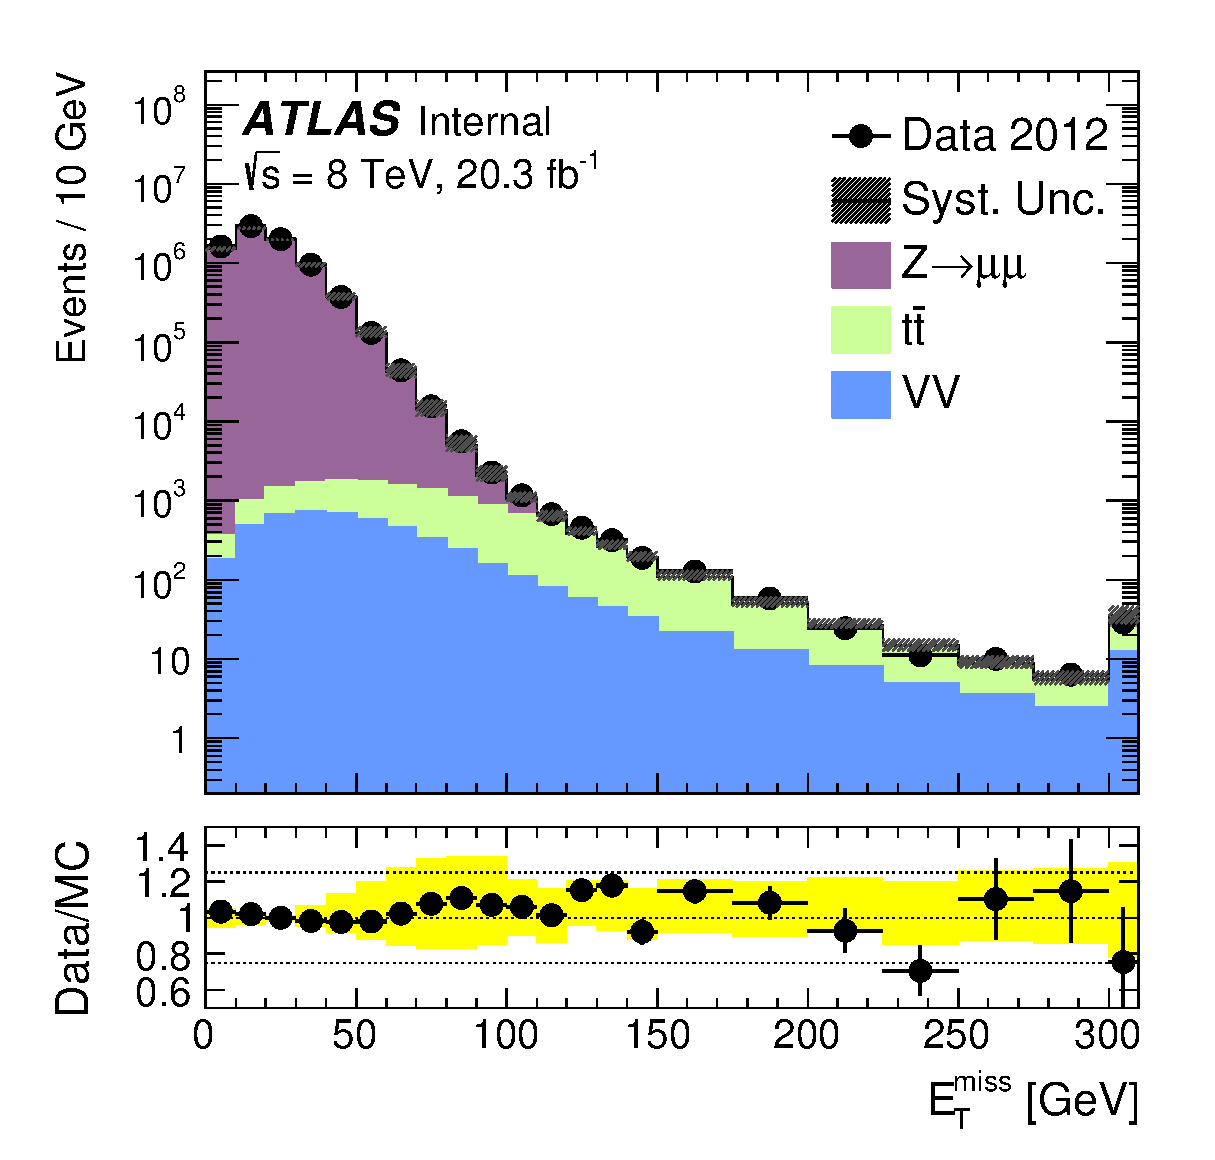
\includegraphics[width=\textwidth]{figures/zmmh_tot_MET.eps}
\caption{\met\ in a $Z\to ll$-rich region in data}
\label{fig:metPerfA}
\end{subfigure} % 
\begin{subfigure}{0.5\textwidth}
   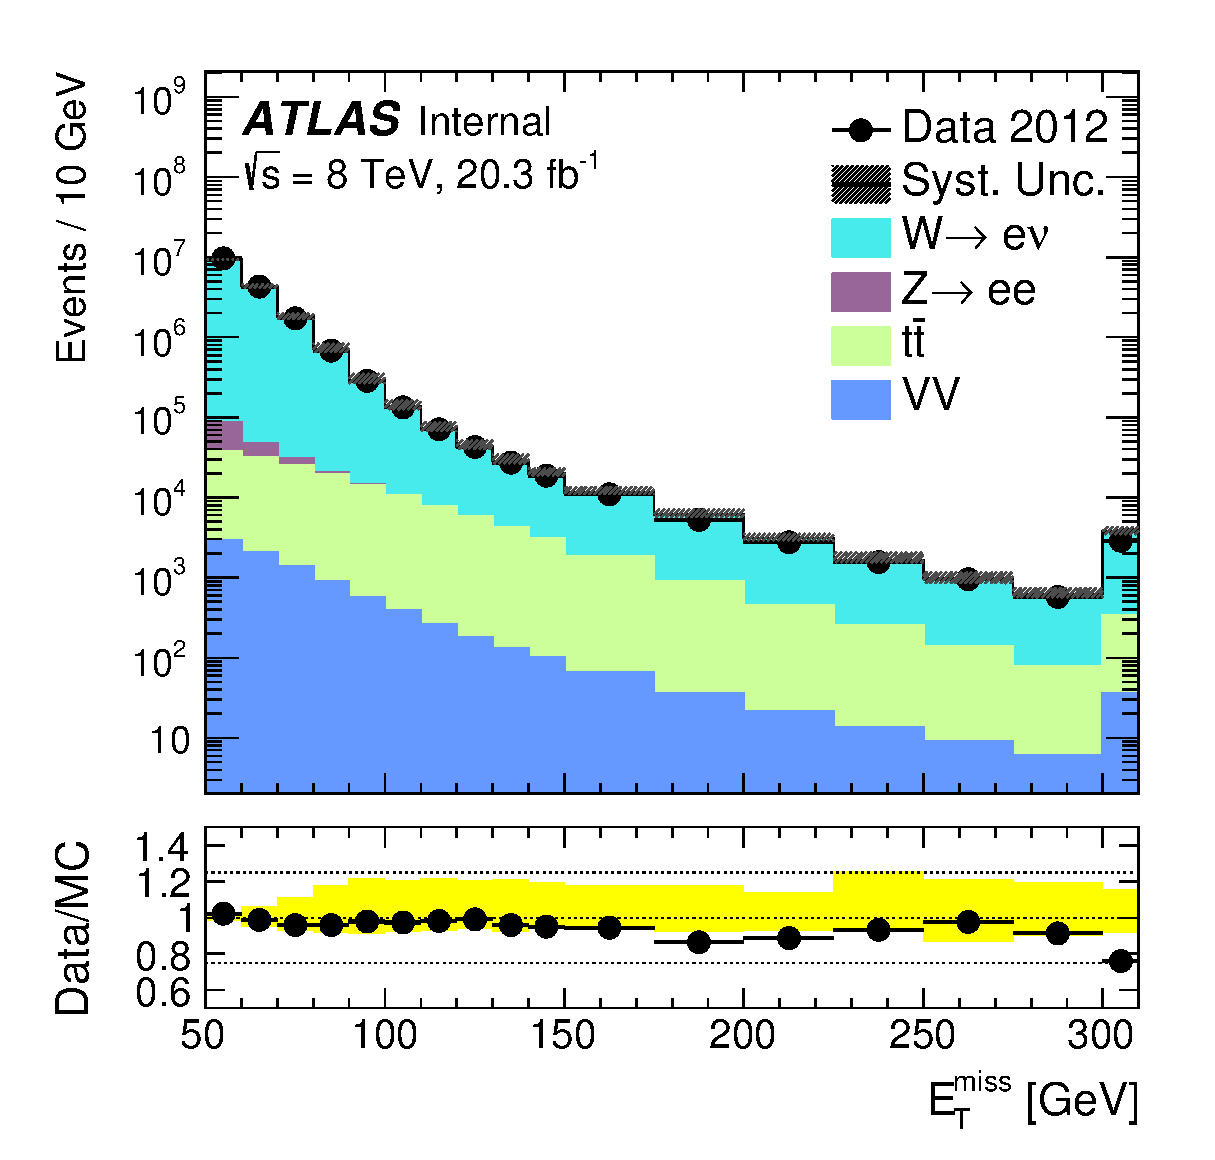
\includegraphics[width=\textwidth]{figures/wenh_tot_MET.eps}
\caption{\met\ in a $W\to l\nu$-rich region in data}
\label{fig:metPerfB}
\end{subfigure}
\caption{Plots showing distributions of \met\ in data, compared to predictions from Monte Carlo distributions, taken from 
Ref~\cite{Khoo:2012749}}
\end{figure}

\par To quantify the \met\ 
performance, its resolution was approximated by the standard deviations 
$\sigma(E^{\text{miss}}_{x(y)} - E^{\text{miss,true}}_{x(y)})$ as functions of $\sum \eT$. 
Since no \met\ was expected in $Z\to ll$ events, these standard deviations were reduced 
to $\sigma(E^{\text{miss}}_{x(y)})$. In $W\to l\nu$ events $E^{\text{miss,true}}_{x(y)})$ 
was obtained from Monte Carlo simulation, so resolutions were studied only in simulation. Contrastingly, in $Z\to ll$ 
events resolutions in data and in Monte Carlo simulation were compared. Either way, these resolutions were observed 
to fall between 5 and 30~\GeV, worsening with increasing $\sum \eT$.

\par Uncertaintiy in the \met\ scale was propagated from the scale uncertainties in the 
individual terms. The uncertainties in the electron, muon, jets, and hadronic $\tau$ terms 
were obtained by methods described in Sections~\ref{sec:ele},~\ref{sec:mu},~\ref{sec:jets}, and 
\ref{sec:tau}. The scale uncertainties in the $E^{\text{miss,softjets}}_{x(y)}$ and $E^{\text{miss,CellOut}}_{x(y)}$ 
terms, collectively known as {\it soft terms}, were evaluated by varying energy 
scales in the topological clusters that contributed to those terms in Monte Carlo 
simulation. After the scale uncertainties from all terms in Equation~\ref{eq:metDef} were evaluated, 
the overall scale uncertainty on \met\ using $W\to l\nu$ Monte Carlo events was found to be 
about 2.6\%. 

\subsection{Run II Reconstruction}
\label{sec:runIImet}
\par The hard terms during Run II reconstruction are formulated just like in Equation~\ref{eq:metDef}.
The selection criteria for the physics objects is however not constant, and consequently \met\ varies 
with the physics object selection. The Run II \met\ used in this thesis is further discussed in 
Section~\ref{sec:objCh}.  

\par To evaluate the perfomance of this reconstruction method a base physics object selection was used. 
The calibration schemes for each of these objects was identical to those used during Run I reconstruction.
Electrons, photons and hadronic $\tau$ leptons were required to not fall in the 
transition region between the central and end-cap calorimeters. 
Electrons were required to be pass the medium selection criteria and have $\pt>10~\GeV$. 
Photons were required to be tightly identified, have $\pt>25~\GeV$. Hadronic $\tau$ leptons 
were required to be of medium quality and have $\pt>20~\GeV$. Muons were required to be of medium 
quality, fall in $|\eta|<2.7$ and have $\pt>10~\GeV$. All jets used had $\pt>20~\GeV$ and $|\eta|>2.4$, or 
$\pt>50~\GeV$ and $|\eta|<4.5$. Any jets with $20<\pt<50~\GeV$ and $|\eta|<2.4$ were required to pass 
additional selection criteria, discussed in Ref~\cite{Brunt:2149445}; other criteria to 
resolve overlaps between objects are also discussed in the same Ref.  

\par The soft term was reconstructed from the \pt\ of tracks in the Inner Detector not associated to any of the 
physics objects discussed in the preceding paragraph. These tracks were required to have at least 
400~\MeV\ in \pt\ and satisfy all track quality criteria discussed in Section~\ref{sec:tracking}.   
In addition, these tracks were required to originate from the primary vertex. This additional requirement 
enabled the soft term to be pileup-robust. 

\subsubsection{Performance and Uncertainties}
\par Performance of \met\ was tested in $Z\to ll$ and $W\to l\nu$ events, just like during 
Run I. Figures~\ref{fig:metPerfrunIIA} and  \ref{fig:metPerfrunIIB} show the \met\ distributions 
in regions in data rich in those two processes respectively. There is reasonable agreement 
between data and Monte Carlo prediction. To quantify this perfomance, the same approximation 
for resolution discussed in Section~\ref{sec:runImet} was used. In $Z\to\mu\mu$ events, resolutions 
obtained in data and Monte Carlo simulations agreed within at most 10\%, with most of the disagreement 
at high $\sum\eT$. The worst resolution was about 20~\GeV\ in both cases. In $W\to \mu\nu$ events   
resolutions were also evaluated with respect to $E^{\text{miss,true}}_{x(y)}$, using Monte Carlo 
simulation. The worst resolution was 25~\GeV.

\begin{figure}[!h]
\begin{subfigure}{0.5\textwidth}
   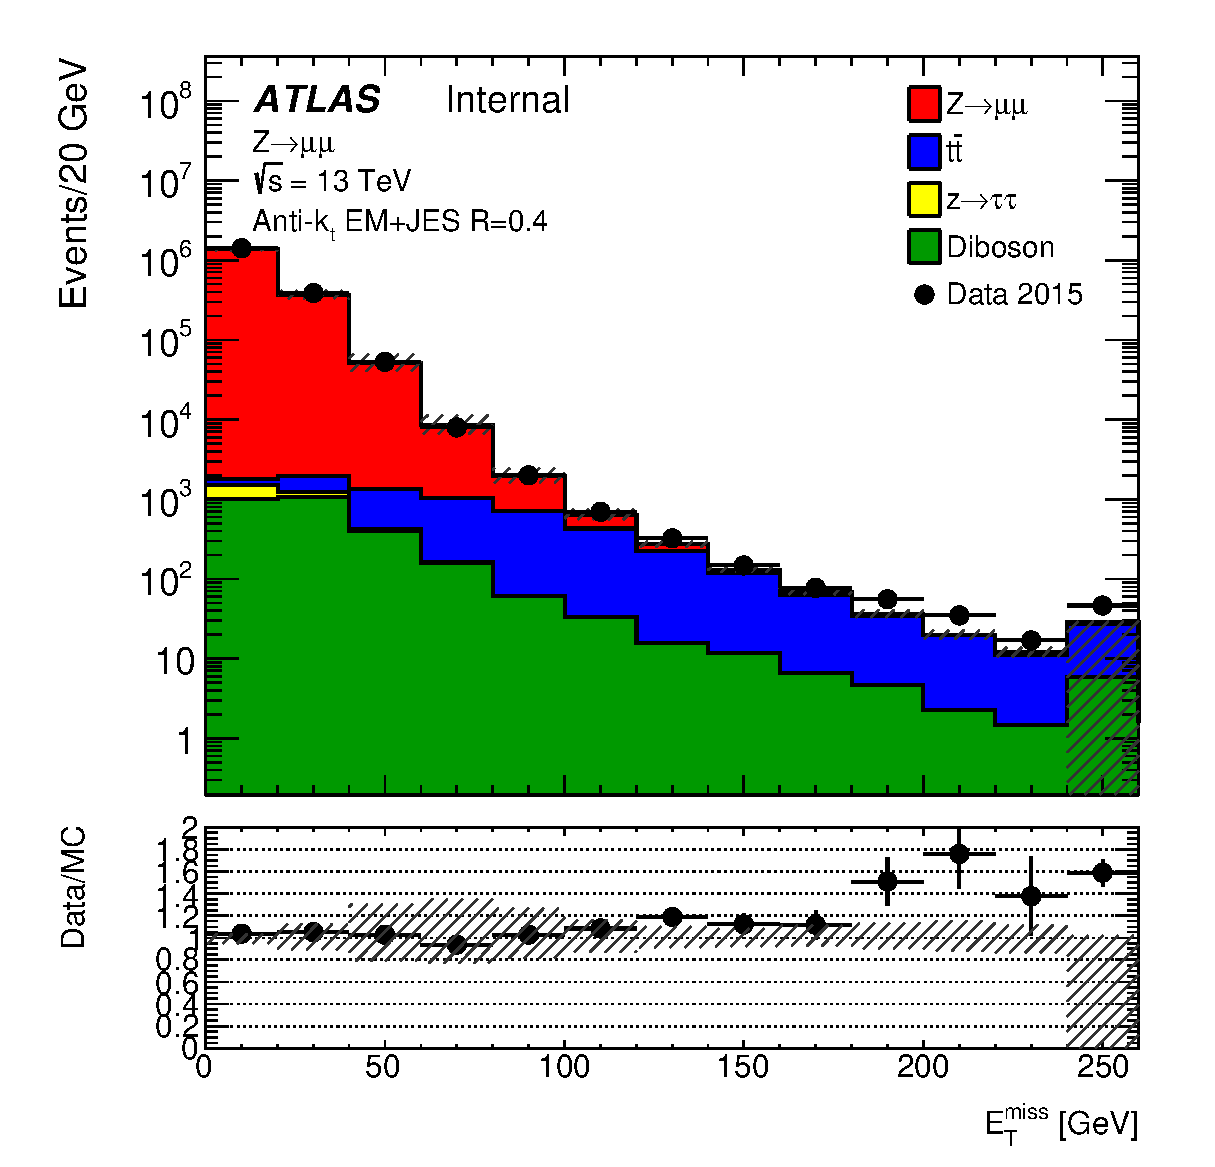
\includegraphics[width=\textwidth]{figures/zmumuStack_met.eps}
\caption{\met\ in a $Z\to ll$-rich region in data}
\label{fig:metPerfrunIIA}
\end{subfigure} % 
\begin{subfigure}{0.5\textwidth}
   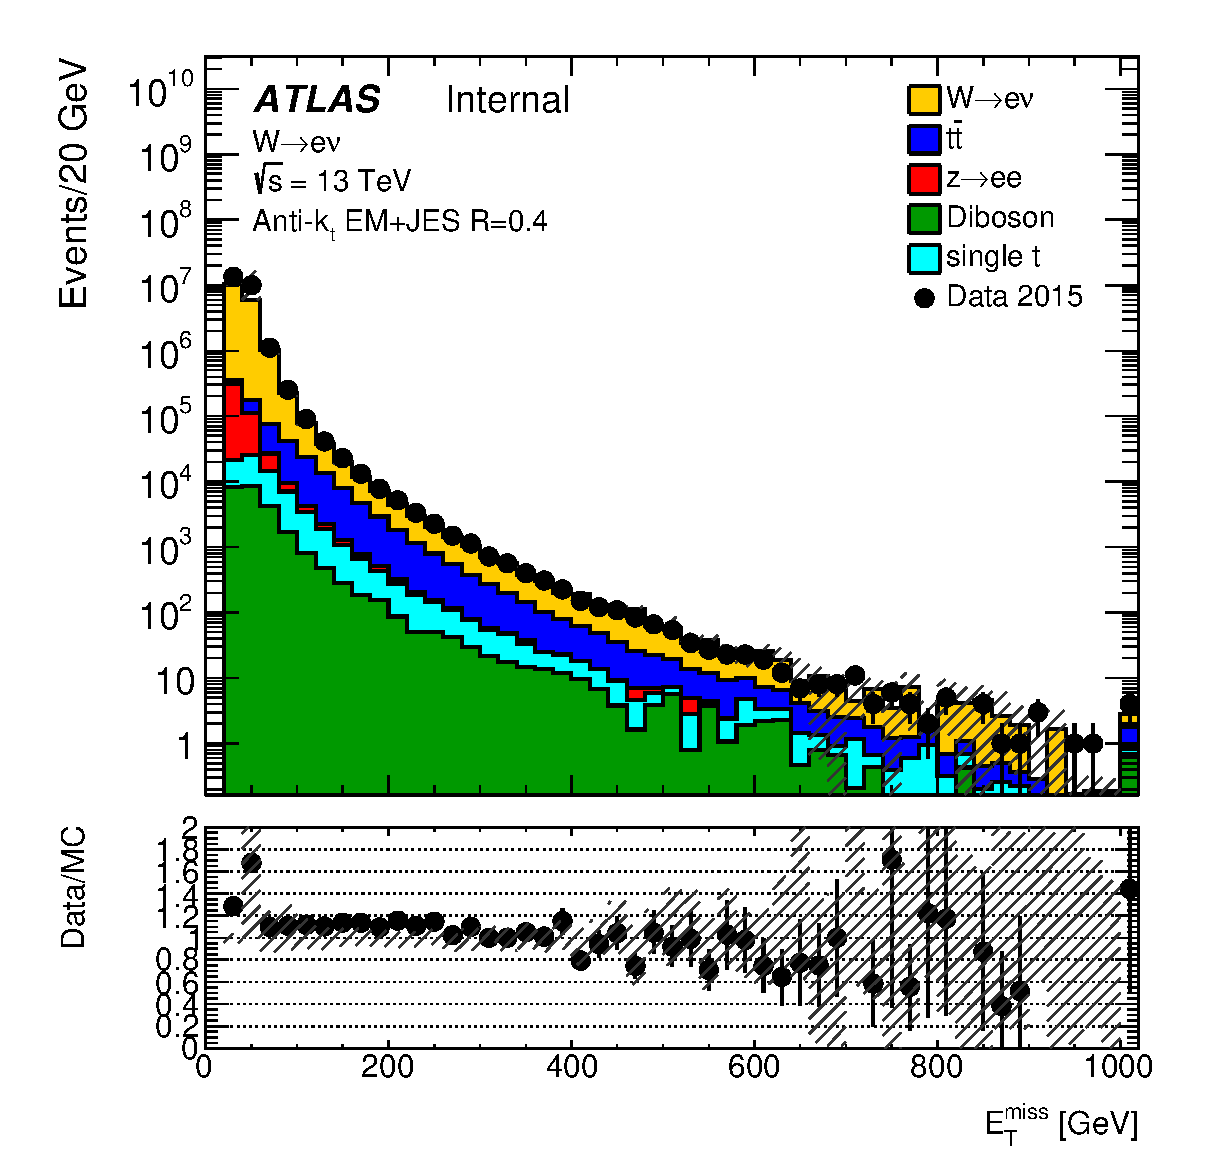
\includegraphics[width=\textwidth]{figures/wenuStack_met.eps}
\caption{\met\ in a $W\to l\nu$-rich region in data}
\label{fig:metPerfrunIIB}
\end{subfigure}
\caption{Plots showing distributions of \met\ in data, compared to predictions from Monte Carlo distributions, taken from 
Ref~\cite{Brunt:2149445}}
\end{figure}

\par Uncertainties on the \met\ scale were determined from comparisons between data and Monte Carlo
simulation. Alternative event generators were used. These were observed to be a few percent~\cite{Brunt:2149445}.
